\subsection{Grundlagen des Protokolls}

Für ein Peer-to-Peer Netzwerk gibt es verschiedene Typen. Abbildung \ref{p2p_typen} zeigt 
vier Typen und ihre Unterteilung in unstrukturierte und strukturierte Netzwerke.

\begin{center}
    \captionsetup{type=figure}
    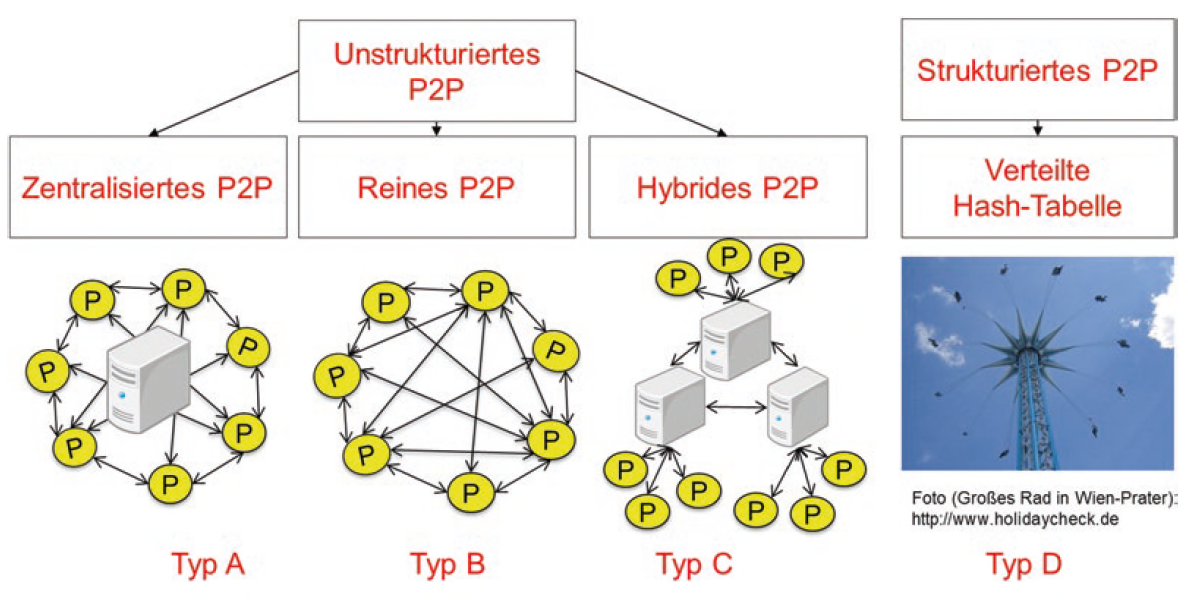
\includegraphics[width=1\linewidth]{images/peer_to_peer_typen.png}
    \captionof{figure}{Typen von Peer-to-Peer Netzwerken \parencite{Luntovskyy_ModRechnernetze}}
    \label{p2p_typen}
\end{center}

\noindent Das Protokoll dieser Arbeit fällt in die Kategorie der hybriden Peer-to-Peer Netzwerke.
Es ist sowohl strukturiert als auch unstrukturiert. In diesem Fall kombiniert die hybride Struktur 
Peer-to-Peer-Kommunikation mit einem zentralen Server als TCP-Relay, um Netzwerkadressübersetzung 
(NAT) zu überwinden. Im Regelfall erfolgt die Kommunikation zwischen den Teilnehmern direkt, ohne dass ein
zentraler Server die Kommunikation steuert. Der zentrale Server wird nur verwendet, um die
Kommunikation zu ermöglichen, wenn die Teilnehmer nicht direkt miteinander kommunizieren können, was 
der Fall ist, wenn die Teilnehmer sich hinter einer Firewall oder einem NAT befinden.
